\chapter{Evaluation}

% IMPORT-DATA algos book1.txt

\begin{figure}[H]
    \centering

    \subfloat[Laufzeiten]{ \scalebox{0.9}{
        \begin{tikzpicture}
            \begin{axis}[
                ybar stacked,
                xtick={1,2,3},
                xticklabels={AreaCompV4/\\LengthFirstArea,RePair,Sequitur},
                xticklabel style={align=center},
                title={Calgary book1 Laufzeit},
                width=7cm,
                y unit={ms},
                ylabel={Laufzeit}
            ]
               
                % PLOT SELECT ROW_NUMBER() OVER(ORDER BY algo ASC) AS x, AVG(comptime) AS y FROM algos GROUP BY algo
                \addplot coordinates { (1,1472.25) (2,7622.75) (3,380.833) };
                % PLOT SELECT ROW_NUMBER() OVER(ORDER BY algo ASC) AS x, AVG(unifytime) AS y FROM algos GROUP BY algo
                \addplot coordinates { (1,353.25) (2,125.75) (3,82.6667) };
                \legend{$Compute$,$Unify$}
                
            \end{axis}
        \end{tikzpicture}
    }}
    \quad
    \subfloat[Kompressionsrate]{ \scalebox{0.9}{
        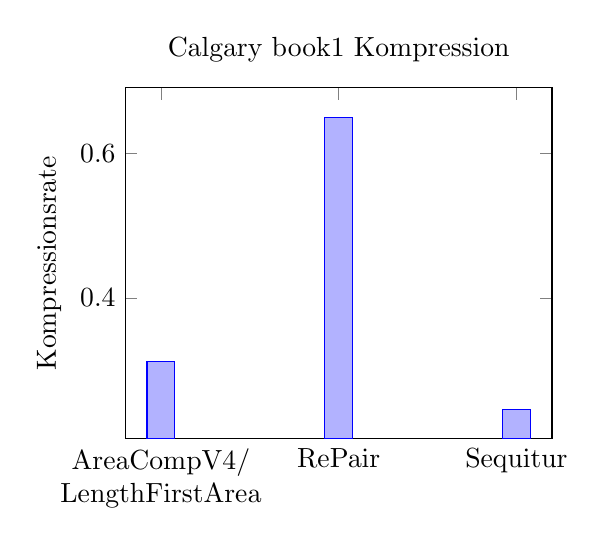
\begin{tikzpicture}
            \begin{axis}[
                ybar stacked,
                xtick={1,2,3},
                xticklabels={AreaCompV4/\\LengthFirstArea,RePair,Sequitur},
                xticklabel style={align=center},
                title={Calgary book1 Kompression},
                width=7cm,
                ylabel={Kompressionsrate}
            ]
                
                % PLOT SELECT ROW_NUMBER() OVER(ORDER BY algo ASC) AS x, MIN(size * 1.0 / inputsize) AS y FROM algos GROUP BY algo
                \addplot coordinates { (1,0.31243) (2,0.65078) (3,0.245433) };
            \end{axis}
        \end{tikzpicture}
    }}
\end{figure}